% latex example

\documentclass[10pt]{article}

   \addtolength{\oddsidemargin} {-0.9in}
   \addtolength{\textwidth}{1.7in}
   \addtolength{\topmargin}{-1.2in}
   \addtolength{\textheight}{2in}
   \linespread{1.1}
   \usepackage{graphicx}
   \usepackage{fancyhdr}
   \usepackage{url}
   \usepackage{amsmath,amssymb}
   \usepackage{comment}
   \pagestyle{fancy}
\lhead{} \chead{} \rhead{} \cfoot{} \rfoot{\thepage}
\renewcommand{\headrulewidth}{0.0pt}
\renewcommand{\footrulewidth}{0.4pt}
\usepackage{xcolor}
\definecolor{mygray}{gray}{0.9}
\usepackage[colorlinks=true,linkcolor=blue,citecolor=blue,urlcolor=blue]{hyperref}
\usepackage{chemmacros}

\usepackage{listings}
\usepackage{color} %red, green, blue, yellow, cyan, magenta, black, white
\definecolor{mygreen}{RGB}{28,172,0} % color values Red, Green, Blue
\definecolor{mylilas}{RGB}{170,55,241}

\lstset{language=Matlab,%
    breaklines=true,%
    morekeywords={matlab2tikz},
    keywordstyle=\color{blue},%
    morekeywords=[2]{1}, keywordstyle=[2]{\color{black}},
    identifierstyle=\color{black},%
    stringstyle=\color{mylilas},
    commentstyle=\color{mygreen},%
    showstringspaces=false,%without this there will be a symbol in the places where there is a space
    numbers=left,%
    numberstyle={\tiny \color{black}},% size of the numbers
    numbersep=9pt, % this defines how far the numbers are from the text
    emph=[1]{for,end,break},emphstyle=[1]\color{red}, %some words to emphasise
}

\begin{document}

\begin{center}
{\Large\bf Homework \#6}\\
 {\bf Name: Andrea Livingston}\\
 {\bf Due: October 28th, 2016}\\
 {\bf CBE660: Intermediate Problems in Chemical and Biological
Engineering\; -\; Fall 2016}\\
Department of Chemical and Biological Engineering, University of Wisconsin-Madison
\end{center}

\noindent\colorbox{mygray}{\begin{minipage}{\textwidth}
  {\bf Problem 1}.  Consider the reversible chemical reaction: 
  \begin{center}
  \ch{A <>[ $k_1$ ][ $k_2$ ] B}  
  \end{center}
 Assume that the reactions are of first-order with constants $k_1,k_2>0$ and denote the concentrations  at time $t$ as $x_A(t)$ and $x_B(t)$. Express the dynamics of this system as $\dot{x}=Ax$ with arbitrary initial concentrations  $x(0)>0$. Address the following:
  \begin{itemize}
  \item If the system is left to react indefinitely, do the concentrations vanish (converge to zero)? Why? 
  \item What type of dynamic response does this system exhibit (damped, damped oscillations, pure oscillations)? 
  \item Prove that the system always settles at a steady-state defined by the eigenvector corresponding to the zero eigenvalue. Based on this insight, answer the following: If your objective is to produce a given chemical using any type of first-order reaction network, does it make sense to design a network that only has negative eigenvalues? 
  \item Implement your eigenvalue decomposition in Matlab (use function {\tt eig} to perform decomposition) and simulate response for $k_1=k_2=1$ and $x(0)=[1\;1]$ over $t\in [0,10]$.  Verify that the system indeed settles at a steady-state defined by the eigenvector with zero eigenvalue. 
   \end{itemize}
\end{minipage}}
\\

{\em Solution:}   
\\ \\
The rate of the chemical reactions can be expressed as
\[\frac{dx_A}{dt}=-k_1x_A+k_2x_B \]
\[\frac{dx_B}{dt}=k_1x_A-k_2x_B \]
Writing this in matrix notation, $\dot{x}=Ax$ gives
\[ \left[ \begin{array}{c} \dot{x}_A \\ \dot{x}_B \end{array} \right] = \left[ \begin{array}{cc} -k_1 & k_2 \\ k_1 & -k_2 \end{array} \right] \left[ \begin{array}{c} x_A \\ x_B \end{array} \right] \]
\\
To find the eigenvalues, we use the property $det(A-\lambda I)=0$
\[(-k_1-\lambda)(-k_2-\lambda)-k_1 k_2=0 \]
\[\lambda^2+\lambda(k_1+k_2)=0 \]
\[\lambda=\frac{-1}{2}(k_1+k_2) \;\pm\; \frac{1}{2}(k_1+k_2) \]
\\
Thus, $\lambda=0$ or $\lambda=-(k_1+k_2)$.
\\ \\
If this system reacts indefinitely, the concentrations go to values defined by the initial condition matrix $x(0)$. It does not make sense for the concentrations to vanish, as mass must be conserved. 
\\ \\
Based on the non-zero eigenvalue, the system has $Re(\lambda)<0$ and $Im(\lambda)=0$ and therefore exhibits damped behavior with no oscillations. 
\\
To find the steady-state solution, we perform a decomposition of matrix A
\\
\[A=S \Lambda S^{-1} \]
\[\dot{x}=Ax=S \Lambda S^{-1} x \]
Let $\dot{y}=S^{-1} \dot{x}$, $y(t)=S^{1}x$ and $y_0=S^{-1}x_0$
\[\dot{y}=\Lambda y(t) \]

\[ \left[ \begin{array}{c} \dot{y}_1 \\ \dot{y}_2 \end{array} \right] = \left[ \begin{array}{cc} \lambda_1 & 0 \\ 0 & \lambda_2 \end{array} \right] \left[ \begin{array}{c} y_1 \\ y_2 \end{array} \right] \]
\\
This yields the solution 
\[ y(t)=e^{\Lambda t}y_0 \]
\\
Using $x(t)=Sy(t)$ and $y_0=S^{-1}x_0$
\[x(t) \;=\; Sy(t) \;=\; Se^{\Lambda t}y_0 \;=\; Se^{\Lambda t}S^{-1}x_0 \]
\\
From the relationship defined above we can prove that the system always settles to the steady-state defined by the eigenvector corresponding to the zero eigenvalue. 

\[ x(t)=S y(t) = \sum_{j=1}^{n} s_j e^{\lambda_j t}s_j^{-1}x_0 \]
\[x(t)=s_1 e^{\lambda_1 t}s_1^{-1}x_0 + s_2 e^{\lambda_2 t}s_2^{-1}x_0 \]
\[x(t)=s_1 e^{0 t}s_1^{-1}x_0 + s_2 e^{-(k_1+k_2) t}s_2^{-1}x_0 \]
\[\lim_{t\to\infty} x(t)=s_1 e^{0}s_1^{-1}x_0 + s_2 e^{-\infty}s_2^{-1}x_0 \]
\[\lim_{t\to\infty} x(t)=s_1 s_1^{-1} x_0 \]
\\
In the limit where $t \rightarrow \infty $ we see that $x(t) \rightarrow s_1 s_1^{-1} x_0$. Therefore the system always settles at the steady state defined by the zero eigenvalue. Note, $s^{-1}$ does not actually exist because you cannot take the inverse of a vector. This notation refers to the vector $s_i$ produced by taking the inverse of the matrix $S$. 
\\ \\
It does not make sense to have exclusively negative eigenvalues for the situation described in the problem statement. In this case, the $x(t) \rightarrow 0$ as $t \rightarrow \infty$ . However, the concentrations cannot all go to zero at steady state because mass must be conserved. \\ 
\\
These results were verified using Matlab. The results and methods are given below.  \\ \\
When $k_1=1$, $k_2=1$ and $x_0=[2,1]$ the system begins at the initial concentrations defined by $x_0$ and converges to the equilibrium concentrations of $x_A=x_B=1.5$. \\ \\
When $k_1=2$, $k_2=1$ and $x_0=[1,1]$ the system begins at the initial concentrations defined by $x_0$ and converges to the equilibrium concentrations of $x_A=~1.3$ and $x_B=~0.7$ Because $k_1$ is defined as twice as large as $k_2$, it is logical that the final concentration of $x_A$ is twice the final concentration of $x_B$. \\ \\

 

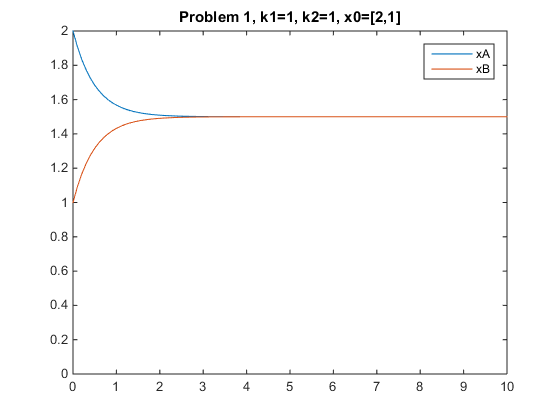
\includegraphics{CBE660_Assign6_1_fig1.png}
\\
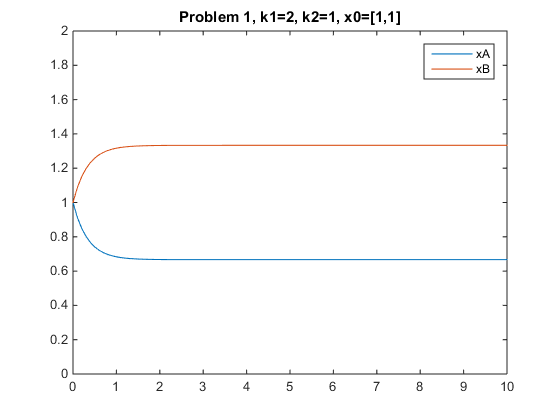
\includegraphics{CBE660_Assign6_1_fig2.png}

\lstinputlisting{CBE660_Assign6_1.m}


\newpage

\noindent\colorbox{mygray}{\begin{minipage}{\textwidth}
  {\bf Problem 2}.  Consider the "loop" reaction network:
    \begin{center}
  \ch{A ->[ $k_1$ ] B}  \\
  \ch{B ->[ $k_2$ ] C}  \\
  \ch{C ->[ $k_3$ ] A}  
  \end{center}
 Assume that the reactions are of first-order with constants $k_1,k_2,k_3\geq 0$ and denote the concentrations  at time $t$ as $x_A(t)$, $x_B(t)$, and $x_C(t)$. Express the dynamics of this system as $\dot{x}=Ax$ with arbitrary initial concentrations  $x(0)>0$. Address the following:
  \begin{itemize}
  \item Assume that the first and third reactions have equal rate constants. Establish a critical value for $k_2$ leading to damped oscillatory behavior.  
  \item Is it possible to find a combination for the rate constants $k_1,k_2,k_3$ (say by designing new catalysts) that make the system oscillate indefinitely? 
   \end{itemize}
  
  \end{minipage}}
\\

{\em Solution:}  
\\
\\
First, the reaction rate expressions can be written in matrix notation
\[ \left[ \begin{array}{c} \dot{x}_A \\ \dot{x}_B \\\dot{x}_C \end{array} \right] = \left[ \begin{array}{ccc} -k_1 & 0 & k_3 \\ k_1 & -k_2 & 0 \\ 0 & k_2 & -k_3 \end{array} \right] \left[ \begin{array}{c} x_A \\ x_B \\x_C \end{array} \right] \]
\\
Use the property $det|A- \lambda I|=0$ to find the eigenvalues
\[(-k_1- \lambda)(-k_2-\lambda)(-k_3-\lambda)+k_1k_2k_3=0 \]
Expanding this expression out, canceling $k_1k_2k_3$  and dividing through by $-\lambda$ yields
\[\lambda^2+\lambda(k_1+k_2+k_3)+k_1k_2+k_1k_3+k_2k_3=0 \]
We can then use the quadratic equation to solve for $\lambda$
\[\lambda=\frac{-b \pm \sqrt{b^2-4ac}}{2a}\]
\[a=1\]
\[b=k_1+k_2+k_3 \]
\[c=k_1k_2+k_1k_3+k_2k_3 \]
\\
To decay with damped oscillations, the $Re(\lambda)<0$ and $Im(\lambda)\neq 0$. Therefore $\frac{-b}{2a}<0$ and $b^2-4ac<0$. The final solution is obtained by allowing $k_1=k_3=K$
\\
From the criteria $Re(\lambda)<0$
\[\frac{b}{a}>0\]
\[k_1+k_2k_3>0 \]
\[2K+k_2>0 \]
\[-k_2<2K\]
\\
From the criteria $Im(\lambda)\neq 0$
\[b^2-4ac<0 \]
\[b^2<4ac \]
\[(k_1+k_2+k_3)^2<4(Kk_2+K^2+Kk_2)\]
\[k_2^2<4Kk_2 \]
\[k_2<4K \]
\\
From the criteria that $Re(\lambda)<0$, we define that $-k_2<2K$. However, because we define in the problem statement that $k_1, k_2, k_3>0$ we know that $2K$ is a positive value and $k_2$ is a positive value. By definition, $-k_2$ will \textit{always} be less that $2K$, regardless of the magnitude of $k_2$. \\
\\
From the criteria that $Im(\lambda) \neq 0$ we see that $k_2<4K$ in order to give a negative within the square root and thus, produce an imaginary component. 
\\
Thus,
\[0 \leq k_2 < 4K \]
\\
It is NOT possible to have a combination that oscillates indefinitely ($Re(\lambda)=0$ and $Im(\lambda) \neq 0$). From the above equations, we can see that for $Re(\lambda)=0$ then $b=k_1+k_2+k_3=0$ must be satisfied. With $k_1, k_2, k_3 \geq 0$, $Re(\lambda)=0$ only when $k_1=k_2=k_3=0$. In this situation, the $Im(\lambda)$ would also be zero, resulting in a system that does not react (straight horizontal line). 

\newpage

\noindent\colorbox{mygray}{\begin{minipage}{\textwidth}
  {\bf Problem 3: When working in the complex domain is the only way to go}.   Consider a linear dynamical system in the Laplace domain $\bar{x}(s)=\bar{f}(s)\bar{u}(s)$ where $\bar{f}(s)$ is its transfer function and $\bar{u}(s)$ is the input (forcing). Recall that the Fourier representation of this system is simply $\bar{x}(j\omega)=\bar{f}(j\omega)\bar{u}(j\omega)$. Address the following:
  \begin{itemize}
\item  Apply the convolution property to $\bar{x}(s)=\bar{f}(s)\bar{u}(s)$ to prove that,  when subjected to a sinusoidal input $u(t)=\sin(\omega t)$, {\em any} dynamical system $\bar{f}(s)$ will ultimately converge to a sinusoidal signal of the form $\lim_{t\to\infty } x(t)= |\bar{f}(j\omega)|\sin(\omega t+\phi)$ where $\phi=\angle \bar{f}(j\omega)$. 
\item Congrats, you just proved one of the most powerful results in control theory. The response $|\bar{f}(j\omega)|\sin(\omega t+\phi)$ is called the ultimate periodic response. This result is useful because we can anticipate the amplitude and phase shift of the response $x(t)$ by knowing the algebraic structure of the transfer function $\bar{f}(j\omega)$. This result is used to estimate unknown parameters of a dynamical system by exciting it using a sinusoidal signal. Now apply your result to the first-order system $\tau\dot{x}(t)+x(t)=Ku(\tau)$ to get an algebraic form of the magnitude and phase shift of the response in terms of the gain $K$ and the time constant $\tau$. 
  \end{itemize}
  \end{minipage}}
\\


{\em Solution:}   
\\
\\
Beginning with the convolution property
\[{\cal L}^{-1}[{\bar f}(s){\bar u}(s)]= \int^t_0 f(t')u(t-t')dt' = x(t) \]
And using the Euler identities
\[e^{j \omega t}=cos(\omega t)+j sin(\omega t) \]
\[e^{-j \omega t}=cos(\omega t)-j sin(\omega t) \]
\[e^{-j \omega t}-e^{j \omega t}=-2jsin(\omega t) \]
\[sin(\omega t)=\frac{-1}{2j}(e^{-j\omega t}-e^{j \omega t}) \]
\\
Substituting this result into $u(t)=sin(\omega t)$ for $t=(t-t')$
\[u(t)=sin(\omega(t-t')) \]
\[x(t)=\int^t_0 f(t')sin(\omega(t-t')) dt' \]
\[x(t)=\int^t_0 f(t')\left[ \frac{-1}{2j}(e^{-j \omega(t-t')}-e^{j \omega (t-t')} ) \right] dt' \]
\[x(t)= 
\int^t_0 f(t')\left[ \frac{-1}{2j}(e^{-j \omega t}e^{j \omega t'} )\right]dt' + 
\int^t_0 f(t')\left[ \frac{-1}{2j}(e^{j \omega t}e^{-j \omega  t'} )\right]dt' \]
\\
Using the Fourier Transform
\[{\bar f}(s)=\int f(t')e^{-j \omega t'}dt' \]
\[x(t)=\frac{1}{2j}e^{j \omega t}{\bar f}(j \omega) - \frac{1}{2j}e^{-j \omega t}{\bar f}(-j \omega) \]
\\
From the properties of the magnitude
\[|{\bar f}(j \omega)|=|{\bar f}(-j \omega)| \]
\[|{\bar f}(j \omega)| = \sqrt{Re({\bar f}(j \omega))^2 + Im({\bar f}(j \omega))^2} \]
\[{\bar f}(j \omega)=|{\bar f}(j \omega)|e^{j \phi} \]
\\
We can substitute this expression into our $x(t)$ to get
\[x(t)=\frac{1}{2j}\left[ e^{j \omega t}|{\bar f}(j \omega)|e^{j \phi}-e^{-j \omega t} |{\bar f}(j \omega)|e^{-j \phi}  \right] \]
\[x(t)=\frac{1}{2j}|{\bar f}(j \omega)| \left[ e^{j(\omega t+\phi)}-e^{-j(\omega t+\phi)} \right] \]
\\
From the Euler identity 
\[sin(s)=\frac{-1}{2j}(e^{-js}-e^{js})\]
\[2jsin(s)=e^{js}-e^{-js} \]
\\
Substituting then gives the final equation
\[x(t)=\frac{1}{2j}|{\bar f}(j \omega)|2jsin(\omega t+\phi) \]
\[x(t)= |{\bar f}(j \omega)| sin(\omega t+\phi) \]
\\
\\
Beginning by taking the Laplace transform of $\tau {\dot x}(t)+x(t)=Ku(t)$
\[ {\cal L}[\tau {\dot x}(t)+x(t)=Ku(\tau)] \longrightarrow \tau(s {\bar x}(s)-{\bar x}(0))+{\bar x}(s)=K{\bar u}(s) \]
\\
Setting $x(0)=0$ and solving for ${\bar x}(s)$
\[{\bar x}(s)(\tau s+1)=K{\bar u}(s) \]
\[{\bar x}(s)=\frac{K}{\tau s+1} {\bar u}(s) \]
\\
To determine the magnitude where $s=j\omega$
\[{\bar f}(j \omega) = \frac{K}{\tau s+1} = \frac{K}{\tau j \omega+1} = \frac{N(j \omega)}{D(j \omega)} \]
\[|{\bar f}(j \omega)|= \frac{K}{|\tau j \omega+1|}= \frac{K}{\sqrt{(\omega \tau)^2+1}} \]
\\
To determine the phase shift
\[\phi = \phi_N- \phi_D \]
\[\phi=tan^{-1}\frac{Im}{Re} \]
\[\phi_N=tan^{-1}(\frac{0}{K}) \]
\[\phi_D=tan^{-1}(\frac{\omega t}{1}) \]
\[\phi=tan^{-1}(\omega t) \]


\newpage


\end{document}


